\documentclass[12pt,a4paper]{article}
\usepackage{amsmath, amssymb, geometry, booktabs, xcolor, hyperref,
            listings, pgfplots, tcolorbox, enumitem, fancyhdr, tikz, array}
\geometry{margin=2.5cm}
\pgfplotsset{compat=1.18}
\tcbuselibrary{skins, breakable}

% ── tcolorbox environments ──────────────────────────────────────────────────
\newtcolorbox{curiositybox}[1]{colback=yellow!10, colframe=orange!80!black,
  fonttitle=\bfseries, title=#1, breakable}
\newtcolorbox{infobox}[1]{colback=blue!5, colframe=blue!60!black,
  fonttitle=\bfseries, title=#1, breakable}
\newtcolorbox{mistakebox}[1]{colback=red!5, colframe=red!60!black,
  fonttitle=\bfseries, title=#1, breakable}
\newtcolorbox{learnbox}[1]{colback=green!5, colframe=green!60!black,
  fonttitle=\bfseries, title=#1, breakable}

% ── lstlisting (Python) ─────────────────────────────────────────────────────
\lstset{language=Python, basicstyle=\ttfamily\small, keywordstyle=\color{blue},
        commentstyle=\color{gray}, stringstyle=\color{orange},
        showstringspaces=false, numbers=left, numberstyle=\tiny,
        breaklines=true, frame=single}

% ── fancyhdr ────────────────────────────────────────────────────────────────
\pagestyle{fancy}
\fancyhf{}
\lhead{Topic 02: Definition of Laplace Transform}
\rhead{Unit IV --- Laplace Transforms}
\cfoot{\thepage}

% ── title ────────────────────────────────────────────────────────────────────
\title{Topic 02: Definition of Laplace Transform \\
       \large Unit IV --- Laplace Transforms}
\author{23A54201 --- Mathematics IV (Transform Techniques) \\
        JNTUA College of Engineering (Autonomous)}
\date{}

% ─────────────────────────────────────────────────────────────────────────────
\begin{document}
\maketitle
\tableofcontents
\newpage

% =============================================================================
\section{Opening Hook}
% =============================================================================
\begin{curiositybox}{Hook}
Every powerful machine needs a precise blueprint. The Laplace Transform is no
exception. Until now, we know \emph{why} it exists --- to convert calculus into
algebra. But \emph{what exactly} is it? It turns out to be a single integral
with a very clever choice of kernel: $e^{-st}$. This one integral, evaluated
from 0 to infinity, encodes everything about $f(t)$ into a new function $F(s)$.
Let's take the blueprint apart, symbol by symbol.
\end{curiositybox}

% =============================================================================
\section{Why This Topic Exists}
% =============================================================================

Before we begin, here is the honest answer to why you are reading this\ldots

Without the formal definition, you are using the Laplace Transform as a black
box --- you can apply it but not derive new results or extend it. The table
below shows what happens when students skip this foundation.

\medskip
\begin{center}
\begin{tabular}{@{}p{7cm} p{7cm}@{}}
\toprule
\textbf{Mistake} & \textbf{Consequence} \\
\midrule
Skipping the definition
  & Unable to compute transforms of non-standard functions \\[4pt]
Confusing $f(t)$ with $F(s)$ notation
  & Writing wrong answers in every subsequent topic \\[4pt]
Not understanding the convergence parameter $s$
  & Missing why $s$ has a lower bound \\[4pt]
Treating the integral as a finite definite integral
  & Arriving at incorrect limits of integration \\[4pt]
Forgetting that $s$ is a parameter, not a variable like $t$
  & Algebraic errors when collecting $s$-terms \\
\bottomrule
\end{tabular}
\end{center}
\medskip

\begin{learnbox}{Why Foundations Matter}
Every formula you will use in Units IV and V descends directly from one
integral. If that integral is clear to you, the rest of the course flows
naturally. Skip it and you will be memorising without understanding.
\end{learnbox}

% =============================================================================
\section{You Already Know This (Intuition First)}
% =============================================================================

Imagine a weighing machine. You place an object --- call it $f(t)$ --- on the
scale. The scale is the integral $\int_0^\infty e^{-st}(\cdot)\,dt$. The
reading on the dial is $F(s)$.

Now here is the key insight: changing the value of $s$ is like switching the
units on the dial from grams to kilograms. You get a different number for each
$s$, but the \emph{object} $f(t)$ has not changed at all. The kernel $e^{-st}$
is the ``calibration knob'' that ensures the reading is finite (convergent) for
suitably large $s$.

This is why $F(s)$ is called a \textbf{transform}: it is the same information
as $f(t)$, re-expressed in a new language. The two domains are genuinely
different --- $t$ is time (measured in seconds), while $s$ has units of
$1/\text{second}$, placing it in the \textbf{frequency domain}.

% =============================================================================
\section{The Formal Definition}
% =============================================================================

\begin{infobox}{Definition of the Laplace Transform}
Let $f(t)$ be a function defined for $t \geq 0$. The \textbf{Laplace
Transform} of $f(t)$ is the function $F(s)$ defined by
\[
  \mathcal{L}\{f(t)\} = F(s) = \int_0^\infty e^{-st}\, f(t)\, dt,
\]
provided the improper integral converges.

\medskip
\noindent\textbf{Symbol-by-symbol unpacking:}
\begin{itemize}[leftmargin=1.5cm]
  \item $f(t)$: the original function, defined for $t \geq 0$ (time domain).
  \item $e^{-st}$: the \emph{damping kernel} --- it forces the integrand to
        decay to zero as $t \to \infty$, ensuring convergence for suitably
        large $s$.
  \item $\int_0^\infty$: an improper integral --- formally the limit
        $\lim_{T \to \infty} \int_0^T e^{-st} f(t)\, dt$.
  \item $F(s)$: the Laplace transform --- a brand-new function of the variable
        $s$ (s-domain).
  \item $s$: a complex parameter; for most B.Tech applications treat it as a
        real positive number.
\end{itemize}

\medskip
Because the transform is built from an integral, it is called an
\textbf{integral transform}. In engineering, the $s$-domain is also called the
\textbf{frequency domain}.
\end{infobox}

\begin{learnbox}{What Did We Learn?}
The Laplace Transform converts a time-domain function $f(t)$ into an
$s$-domain function $F(s)$ via a single improper integral with exponential
kernel $e^{-st}$. The parameter $s$ must be large enough to guarantee
convergence.
\end{learnbox}

% =============================================================================
\section{Notation Conventions}
% =============================================================================

\begin{infobox}{Strict Notation Rules Used Throughout This Course}
\begin{itemize}[leftmargin=1.5cm]
  \item Time-domain functions use \textbf{lowercase}: $f(t)$, $g(t)$, $y(t)$.
  \item Transform-domain functions use \textbf{uppercase}: $F(s)$, $G(s)$,
        $Y(s)$.
  \item The transform operator is always written as $\mathcal{L}\{f(t)\}$ ---
        use the calligraphic $\mathcal{L}$, \emph{never} the plain letter $L$.
  \item Transform pair notation:
        $f(t) \xleftrightarrow{\mathcal{L}} F(s)$.
\end{itemize}

\medskip
\noindent\textbf{Common notation errors and their corrections:}

\medskip
\begin{center}
\begin{tabular}{@{}ll@{}}
\toprule
\textbf{Incorrect Notation} & \textbf{Correct Notation} \\
\midrule
$L\{f(t)\}$ & $\mathcal{L}\{f(t)\}$ \\[3pt]
$\mathcal{L}\{F(t)\}$ & $\mathcal{L}\{f(t)\}$ (use lowercase for time domain) \\[3pt]
$f(s)$ as the transform result & $F(s)$ (uppercase for $s$-domain) \\[3pt]
$F(t)$ for the transform & $F(s)$ (the transform is a function of $s$, not $t$) \\[3pt]
$\mathcal{L}(f(t))$ (round brackets) & $\mathcal{L}\{f(t)\}$ (curly braces) \\[3pt]
$\mathcal{L}^{-1}(F(s))$ & $\mathcal{L}^{-1}\{F(s)\}$ (curly braces here too) \\[3pt]
$L^{-1}\{F(s)\}$ & $\mathcal{L}^{-1}\{F(s)\}$ (calligraphic always) \\
\bottomrule
\end{tabular}
\end{center}
\end{infobox}

\begin{learnbox}{What Did We Learn?}
Notation is not cosmetic. Mixing uppercase and lowercase, or using plain $L$
instead of $\mathcal{L}$, leads to wrong answers that are impossible to track
down later. Commit these conventions now.
\end{learnbox}

% =============================================================================
\section{Linearity of the Laplace Transform}
% =============================================================================

\begin{infobox}{Linearity Property --- Statement and Proof}
\textbf{Theorem (Linearity).} Let $f(t)$ and $g(t)$ be functions whose Laplace
transforms exist, and let $a, b$ be any constants. Then
\[
  \mathcal{L}\{a\,f(t) + b\,g(t)\} = a\,\mathcal{L}\{f(t)\} + b\,\mathcal{L}\{g(t)\}
  = a\,F(s) + b\,G(s).
\]

\medskip
\textbf{Proof (directly from the definition):}

Starting from the definition,
\begin{align*}
  \mathcal{L}\{a\,f(t) + b\,g(t)\}
  &= \int_0^\infty e^{-st}\bigl[a\,f(t) + b\,g(t)\bigr]\, dt \\
  &= \int_0^\infty \bigl[a\,e^{-st} f(t) + b\,e^{-st} g(t)\bigr]\, dt
     && \text{(distribute $e^{-st}$)} \\
  &= a \int_0^\infty e^{-st} f(t)\, dt + b \int_0^\infty e^{-st} g(t)\, dt
     && \text{(linearity of the integral)} \\
  &= a\,F(s) + b\,G(s).
     && \text{(definition applied twice)}
\end{align*}
\qed

\medskip
\textbf{Why linearity matters.} Any linear combination of functions ---
such as $3e^{2t} - 5\cos t + 7$ --- can be split into individual pieces,
each transformed separately, then the results added. This is the engine
behind every table of transforms you will use in this course.
\end{infobox}

\begin{learnbox}{What Did We Learn?}
Linearity means ``break, transform, and add.'' It is the reason a short
table of basic transforms is enough to handle enormously complicated functions.
\end{learnbox}

% =============================================================================
\section{First Direct Computations}
% =============================================================================

\begin{infobox}{Derivation 1 --- $\mathcal{L}\{1\}$}
We compute directly from the definition:
\begin{align*}
  \mathcal{L}\{1\}
  &= \int_0^\infty e^{-st} \cdot 1\, dt \\
  &= \lim_{T \to \infty} \int_0^T e^{-st}\, dt \\
  &= \lim_{T \to \infty} \left[\frac{e^{-st}}{-s}\right]_0^T \\
  &= \lim_{T \to \infty} \left(\frac{e^{-sT}}{-s} - \frac{e^{0}}{-s}\right) \\
  &= \lim_{T \to \infty} \left(-\frac{e^{-sT}}{s} + \frac{1}{s}\right).
\end{align*}
Since $s > 0$, we have $e^{-sT} \to 0$ as $T \to \infty$. Therefore
\[
  \mathcal{L}\{1\} = \frac{1}{s}, \qquad s > 0.
\]
\end{infobox}

\begin{learnbox}{What Did We Learn?}
The constant function 1 transforms to $1/s$. The condition $s > 0$ is
necessary: if $s \leq 0$ the exponential $e^{-sT}$ would not decay to zero
and the integral would diverge.
\end{learnbox}

\begin{infobox}{Derivation 2 --- $\mathcal{L}\{e^{at}\}$}
\begin{align*}
  \mathcal{L}\{e^{at}\}
  &= \int_0^\infty e^{-st} e^{at}\, dt \\
  &= \int_0^\infty e^{-(s-a)t}\, dt \\
  &= \lim_{T \to \infty} \int_0^T e^{-(s-a)t}\, dt \\
  &= \lim_{T \to \infty} \left[\frac{e^{-(s-a)t}}{-(s-a)}\right]_0^T \\
  &= \lim_{T \to \infty} \left(-\frac{e^{-(s-a)T}}{s-a} + \frac{1}{s-a}\right).
\end{align*}
For the limit to be zero we need $s - a > 0$, i.e.\ $s > a$. Under that
condition $e^{-(s-a)T} \to 0$, giving
\[
  \mathcal{L}\{e^{at}\} = \frac{1}{s - a}, \qquad s > a.
\]
\textbf{Why $s > a$?} If $s \leq a$ then $e^{-(s-a)t} = e^{|s-a|t}$ grows
without bound and the integral diverges. The condition $s > a$ is the
\emph{convergence strip} for this transform.
\end{infobox}

\begin{learnbox}{What Did We Learn?}
$\mathcal{L}\{e^{at}\} = 1/(s-a)$ for $s > a$. The sign in the denominator
is $s - a$ (minus), \emph{not} $s + a$. This is the single most common sign
error in this course.
\end{learnbox}

\begin{infobox}{Derivation 3 --- $\mathcal{L}\{t\}$}
\begin{align*}
  \mathcal{L}\{t\}
  &= \int_0^\infty e^{-st}\, t\, dt.
\end{align*}
We apply integration by parts. Let $u = t$ and $dv = e^{-st}\, dt$. Then
$du = dt$ and $v = -\tfrac{1}{s}e^{-st}$. Therefore
\begin{align*}
  \int_0^\infty t\, e^{-st}\, dt
  &= \left[t \cdot \left(-\frac{e^{-st}}{s}\right)\right]_0^\infty
     - \int_0^\infty \left(-\frac{e^{-st}}{s}\right) dt \\[4pt]
  &= \left[-\frac{t\, e^{-st}}{s}\right]_0^\infty
     + \frac{1}{s}\int_0^\infty e^{-st}\, dt.
\end{align*}
Evaluate the boundary term: as $t \to \infty$ with $s > 0$,
$t\,e^{-st} \to 0$ (exponential dominates the linear factor); at $t = 0$,
$t\,e^{-st} = 0$. So the boundary term is $0 - 0 = 0$. For the remaining
integral we already know $\int_0^\infty e^{-st}\, dt = 1/s$. Hence
\[
  \mathcal{L}\{t\} = 0 + \frac{1}{s} \cdot \frac{1}{s} = \frac{1}{s^2},
  \qquad s > 0.
\]
\end{infobox}

\begin{learnbox}{What Did We Learn?}
Integration by parts is the standard technique for transforms of polynomial
terms. The boundary term vanishes because the exponential $e^{-st}$ decays
faster than any power of $t$ grows --- a fact that will recur throughout
this course.
\end{learnbox}

% =============================================================================
\section{Visualizing the Transform}
% =============================================================================

The two plots below illustrate the same ``information'' expressed in two
completely different domains. The left plot shows $f(t) = e^{-2t}$ in the
time domain; the right shows its Laplace transform $F(s) = \tfrac{1}{s+2}$
in the $s$-domain.

\medskip
\begin{center}
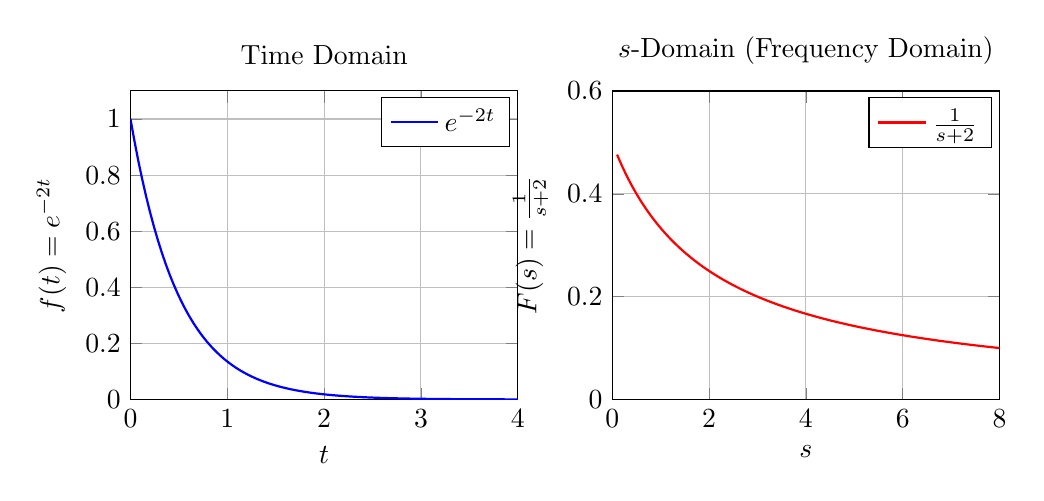
\begin{tikzpicture}
  % ── Left axis: time domain ──────────────────────────────────────────────
  \begin{axis}[
    name=leftplot,
    width=6.5cm, height=5.5cm,
    xlabel={$t$}, ylabel={$f(t) = e^{-2t}$},
    xmin=0, xmax=4, ymin=0, ymax=1.1,
    grid=major,
    title={Time Domain},
    xtick={0,1,2,3,4},
    ytick={0,0.2,0.4,0.6,0.8,1.0},
  ]
    \addplot[blue, thick, domain=0:4, samples=100] {exp(-2*x)};
    \addlegendentry{$e^{-2t}$}
  \end{axis}

  % ── Right axis: s-domain ───────────────────────────────────────────────
  \begin{axis}[
    at={(leftplot.east)}, anchor=west, xshift=1.2cm,
    width=6.5cm, height=5.5cm,
    xlabel={$s$}, ylabel={$F(s) = \frac{1}{s+2}$},
    xmin=0, xmax=8, ymin=0, ymax=0.6,
    grid=major,
    title={$s$-Domain (Frequency Domain)},
    xtick={0,2,4,6,8},
  ]
    \addplot[red, thick, domain=0.1:8, samples=200] {1/(x+2)};
    \addlegendentry{$\frac{1}{s+2}$}
  \end{axis}
\end{tikzpicture}
\end{center}

\medskip
\noindent\textit{Caption: The same ``information'' lives in both plots ---
but $F(s)$ is not a plot of $f(t)$ vs.\ $s$. They are completely different
functions in completely different domains.}

\begin{learnbox}{What Did We Learn?}
The time-domain plot shows exponential decay. The $s$-domain plot shows a
hyperbola decreasing toward zero. Both encode the same physical signal; the
Laplace Transform simply re-expresses it in a form that makes algebra easier.
\end{learnbox}

% =============================================================================
\section{Worked Examples}
% =============================================================================

\begin{infobox}{Example 1 --- $\mathcal{L}\{5 - 3e^{2t}\}$}
\textbf{Objective:} Use linearity and the results of Section~7 to compute this
transform without re-deriving from first principles.

\medskip
\textbf{Step 1.} Apply linearity:
\[
  \mathcal{L}\{5 - 3e^{2t}\}
  = \mathcal{L}\{5 \cdot 1\} + \mathcal{L}\{(-3)\,e^{2t}\}
  = 5\,\mathcal{L}\{1\} - 3\,\mathcal{L}\{e^{2t}\}.
\]

\textbf{Step 2.} Substitute the known results ($a = 0$ for the constant, $a = 2$ for the exponential):
\[
  = 5 \cdot \frac{1}{s} - 3 \cdot \frac{1}{s - 2}.
\]

\textbf{Step 3.} Combine over a common denominator:
\[
  = \frac{5(s-2) - 3s}{s(s-2)}
  = \frac{5s - 10 - 3s}{s(s-2)}
  = \frac{2s - 10}{s(s-2)}.
\]

\textbf{Convergence condition:} The transform of $e^{2t}$ requires $s > 2$,
which is the binding constraint. The transform of the constant 1 requires
only $s > 0$. Therefore the combined result is valid for $s > 2$.

\[
  \boxed{\mathcal{L}\{5 - 3e^{2t}\} = \frac{2s-10}{s(s-2)}, \quad s > 2.}
\]
\end{infobox}

\begin{learnbox}{What Did We Learn?}
When computing the transform of a linear combination, always: (1) split by
linearity, (2) apply known results, (3) state the convergence condition as the
\emph{most restrictive} condition among the individual terms.
\end{learnbox}

\begin{infobox}{Example 2 --- $\mathcal{L}\{e^{-t} + 4\}$}
\textbf{Step 1.} Apply linearity:
\[
  \mathcal{L}\{e^{-t} + 4\}
  = \mathcal{L}\{e^{-t}\} + 4\,\mathcal{L}\{1\}.
\]

\textbf{Step 2.} Use $\mathcal{L}\{e^{at}\} = \tfrac{1}{s-a}$ with $a = -1$:
\[
  \mathcal{L}\{e^{-t}\} = \frac{1}{s-(-1)} = \frac{1}{s+1}, \quad s > -1.
\]
And $\mathcal{L}\{1\} = \tfrac{1}{s}$ for $s > 0$.

\textbf{Step 3.} Combine:
\[
  \mathcal{L}\{e^{-t} + 4\}
  = \frac{1}{s+1} + \frac{4}{s}
  = \frac{s + 4(s+1)}{s(s+1)}
  = \frac{5s + 4}{s(s+1)}.
\]

\textbf{Convergence condition:} $s > 0$ is the binding constraint (more
restrictive than $s > -1$).

\[
  \boxed{\mathcal{L}\{e^{-t} + 4\} = \frac{5s+4}{s(s+1)}, \quad s > 0.}
\]
\end{infobox}

\begin{learnbox}{What Did We Learn?}
When $a$ is negative (here $a = -1$), the formula $1/(s-a)$ gives
$1/(s+1)$ --- the denominator becomes $s$ \emph{plus} a positive number.
Always substitute the sign of $a$ explicitly rather than memorising by
pattern.
\end{learnbox}

\begin{infobox}{Example 3 --- Identifying a Sign Error}
\textbf{Problem.} A student writes
\[
  \mathcal{L}\{e^{at}\} = \frac{1}{s + a}.
\]
Identify the error and give the correct answer.

\medskip
\textbf{Error identification.} The student has written $s + a$ in the
denominator. The correct derivation (see Section~7, Derivation~2) shows that
the combined exponent in the integral is $-(s-a)t$, giving denominator
$(s - a)$. Writing $s + a$ is equivalent to claiming the exponent is
$-(s+a)t$, which corresponds to the transform of $e^{-at}$, not $e^{at}$.

\medskip
\textbf{Where the error likely comes from.} Students remember the exponential
``goes to the bottom'' and place the letter $a$ after $s$ without tracking the
sign. The safest method: always merge the two exponentials first:
$e^{-st} \cdot e^{at} = e^{-(s-a)t}$, and then integrate directly.

\medskip
\textbf{Correct answer:}
\[
  \mathcal{L}\{e^{at}\} = \frac{1}{s - a}, \qquad s > a.
\]
\end{infobox}

\begin{learnbox}{What Did We Learn?}
The denominator for $\mathcal{L}\{e^{at}\}$ is always $s - a$ (minus), never
$s + a$. A quick sanity check: at $a = 0$ the formula should reduce to
$1/(s-0) = 1/s = \mathcal{L}\{1\}$, which is correct.
\end{learnbox}

% =============================================================================
\section{Excel Example}
% =============================================================================

\textbf{Objective:} Numerically verify that $\mathcal{L}\{e^{-2t}\}$ at
$s = 5$ equals $1/(5+2) = 1/7 \approx 0.1429$.

\medskip
The integral to approximate is
\[
  \int_0^\infty e^{-5t} \cdot e^{-2t}\, dt = \int_0^\infty e^{-7t}\, dt.
\]
We discretise from $t = 0$ to $t = 5$ in steps of $h = 0.5$ and apply the
\textbf{trapezoid rule}:
\[
  \text{Area} \approx \frac{h}{2}\bigl[f(t_0) + 2f(t_1) + \cdots + 2f(t_{n-1}) + f(t_n)\bigr].
\]

\medskip
\begin{center}
\begin{tabular}{@{}ccc@{}}
\toprule
\textbf{Column A} & \textbf{Column B} & \textbf{Column C} \\
$t$ & $e^{-5t} \cdot e^{-2t}$ & Cumulative Trapezoid Area \\
\midrule
\texttt{0}    & \texttt{=EXP(-5*A2)*EXP(-2*A2)}  & (start at 0) \\
\texttt{0.5}  & \texttt{=EXP(-5*A3)*EXP(-2*A3)}  & \texttt{=C2+(A3-A2)/2*(B2+B3)} \\
\texttt{1.0}  & \texttt{=EXP(-5*A4)*EXP(-2*A4)}  & \texttt{=C3+(A4-A3)/2*(B3+B4)} \\
\texttt{1.5}  & \texttt{=EXP(-5*A5)*EXP(-2*A5)}  & \texttt{=C4+(A5-A4)/2*(B4+B5)} \\
\texttt{2.0}  & \texttt{=EXP(-5*A6)*EXP(-2*A6)}  & \texttt{=C5+(A6-A5)/2*(B5+B6)} \\
\texttt{2.5}  & \texttt{=EXP(-5*A7)*EXP(-2*A7)}  & \texttt{=C6+(A7-A6)/2*(B6+B7)} \\
\texttt{3.0}  & \texttt{=EXP(-5*A8)*EXP(-2*A8)}  & \texttt{=C7+(A8-A7)/2*(B7+B8)} \\
\texttt{3.5}  & \texttt{=EXP(-5*A9)*EXP(-2*A9)}  & \texttt{=C8+(A9-A8)/2*(B8+B9)} \\
\texttt{4.0}  & \texttt{=EXP(-5*A10)*EXP(-2*A10)} & \texttt{=C9+(A10-A9)/2*(B9+B10)} \\
\texttt{4.5}  & \texttt{=EXP(-5*A11)*EXP(-2*A11)} & \texttt{=C10+(A11-A10)/2*(B10+B11)} \\
\texttt{5.0}  & \texttt{=EXP(-5*A12)*EXP(-2*A12)} & \texttt{=C11+(A12-A11)/2*(B11+B12)} \\
\bottomrule
\end{tabular}
\end{center}

\medskip
\noindent\textbf{How to interpret the spreadsheet:}
Column B evaluates $e^{-7t}$ at each row (note: \texttt{EXP(-5*A2)*EXP(-2*A2)}
$= e^{-7 \times 0} = 1$ at $t=0$, and approaches 0 rapidly).
Column C accumulates the trapezoid area strip by strip.
At $t = 5$ the cumulative area in cell C12 will read approximately
$\mathbf{0.1429}$, matching the exact value.

\begin{learnbox}{What Did We Learn?}
The trapezoid sum from $t = 0$ to $t = 5$ gives $\approx 0.1429$, confirming
the analytical result $\mathcal{L}\{e^{-2t}\}\big|_{s=5} = 1/7 \approx 0.1429$.
The tail beyond $t = 5$ contributes less than $e^{-35} \approx 6 \times 10^{-16}$
and is negligible. Numerical verification builds confidence in symbolic results.
\end{learnbox}

% =============================================================================
\section{Python Example}
% =============================================================================

The script below uses \texttt{sympy} to compute the Laplace Transform
symbolically from the definition integral for three functions.

\begin{lstlisting}[language=Python, caption={Symbolic Laplace Transform via SymPy}]
from sympy import *

t, s, a = symbols('t s a', real=True, positive=True)

# Helper: integrate e^{-st} * f(t) from 0 to infinity
def laplace_from_def(f):
    return integrate(exp(-s*t) * f, (t, 0, oo))

# 1. f(t) = 1
f1 = S(1)
F1 = laplace_from_def(f1)
print("L{1} =", F1)                     # Expected: 1/s

# 2. f(t) = e^{at}
f2 = exp(a*t)
F2 = laplace_from_def(f2)
print("L{e^(at)} =", simplify(F2))      # Expected: 1/(s - a)

# 3. f(t) = t
f3 = t
F3 = laplace_from_def(f3)
print("L{t} =", F3)                     # Expected: 1/s**2

# Verify numerically at s=5, a=2 for e^{at}
F2_val = F2.subs([(s, 5), (a, 2)])
print("L{e^(2t)} at s=5 =", F2_val)     # Expected: 1/3
\end{lstlisting}

\medskip
\noindent\textbf{Expected output:}
\begin{verbatim}
L{1} = 1/s
L{e^(at)} = 1/(s - a)
L{t} = s**(-2)
L{e^(2t)} at s=5 = 1/3
\end{verbatim}

\begin{learnbox}{What Did We Learn?}
SymPy confirms all three derivations: $1/s$, $1/(s-a)$, and $1/s^2$.
The numerical substitution $s=5$, $a=2$ gives $1/(5-2)=1/3$ --- a quick
sanity check you can perform for any formula. SymPy's \texttt{integrate}
with \texttt{oo} correctly handles the improper integral as the limit
$T \to \infty$.
\end{learnbox}

% =============================================================================
\section{Viva-Style Oral Questions}
% =============================================================================

\begin{enumerate}[leftmargin=1.5cm, label=\textbf{Q\arabic*.}]

  \item \textbf{State the formal definition of the Laplace Transform.}

  \textit{Answer.}
  $\mathcal{L}\{f(t)\} = F(s) = \int_0^\infty e^{-st} f(t)\, dt$, provided
  the improper integral converges. Here $t \geq 0$ is the time variable and
  $s$ is a complex parameter (treated as real and positive in most B.Tech
  applications).

  \item \textbf{What does the term ``s-domain'' (or frequency domain) mean?}

  \textit{Answer.}
  The $s$-domain is the space in which the transformed function $F(s)$ lives.
  After applying the Laplace Transform, the independent variable changes from
  time $t$ (measured in seconds) to the parameter $s$ (measured in
  $1/\text{second}$). In electrical engineering, $s$ generalises the concept
  of frequency, which is why the $s$-domain is also called the frequency domain.

  \item \textbf{Why is the lower limit of the Laplace integral 0, not
        $-\infty$?}

  \textit{Answer.}
  By convention, the Laplace Transform is designed for \emph{causal} systems
  --- systems that are ``switched on'' at time $t = 0$ and have no history
  before that moment. Setting the lower limit to 0 encodes this assumption.
  Functions defined for all $t$ (including $t < 0$) are handled by the
  bilateral Laplace Transform, which is a separate (more advanced) topic.

  \item \textbf{What is the role of the kernel $e^{-st}$?}

  \textit{Answer.}
  The kernel $e^{-st}$ is an exponential damping factor. For $s > 0$ it
  forces the integrand $e^{-st} f(t)$ to decay to zero as $t \to \infty$,
  thereby guaranteeing that the improper integral converges even when $f(t)$
  itself grows (e.g.\ $f(t) = e^{2t}$, provided $s > 2$). Without this
  kernel, most engineering functions would yield a divergent integral.

  \item \textbf{What is the notation convention for time-domain versus
        s-domain functions?}

  \textit{Answer.}
  The convention is: lowercase letters for time-domain functions
  ($f(t)$, $g(t)$, $y(t)$) and the corresponding uppercase letters for their
  Laplace transforms ($F(s)$, $G(s)$, $Y(s)$). The transform operator is
  always written as $\mathcal{L}$ (calligraphic), never as the plain letter
  $L$.

  \item \textbf{State and prove the linearity property of the Laplace
        Transform.}

  \textit{Answer.}
  \textbf{Statement:} $\mathcal{L}\{af(t) + bg(t)\} = aF(s) + bG(s)$.
  \textbf{Proof:} Apply the definition, distribute $e^{-st}$, then use the
  linearity of the Riemann integral to split into two integrals, each of which
  equals $a\,F(s)$ and $b\,G(s)$ respectively by definition. (See Section~6
  for the full proof.)

  \item \textbf{Why does $\mathcal{L}\{e^{at}\} = \tfrac{1}{s-a}$ require
        $s > a$?}

  \textit{Answer.}
  After combining the two exponentials, the integrand becomes $e^{-(s-a)t}$.
  For this to decay to zero as $t \to \infty$ we need the exponent
  $-(s-a)t \to -\infty$, which requires $s - a > 0$, i.e.\ $s > a$.
  If $s \leq a$ the integrand grows or stays constant, making the improper
  integral diverge.

  \item \textbf{What is the improper integral $\int_0^\infty$ as a limit?}

  \textit{Answer.}
  The improper integral is defined as
  $\int_0^\infty f(t)\, dt = \lim_{T \to \infty} \int_0^T f(t)\, dt$.
  We first evaluate the ordinary definite integral from 0 to a finite upper
  limit $T$, and then take the limit as $T \to \infty$. The transform exists
  if and only if this limit is finite.

\end{enumerate}

% =============================================================================
\section{Descriptive Questions}
% =============================================================================

\begin{enumerate}[leftmargin=1.5cm, label=\textbf{D\arabic*.}]

  \item \textbf{State and explain the formal definition of the Laplace
        Transform.}
  Define $\mathcal{L}\{f(t)\} = \int_0^\infty e^{-st} f(t)\, dt$.
  Explain the role of each symbol: $f(t)$ (time-domain function), $e^{-st}$
  (damping kernel), the improper integral (limit as upper bound $\to \infty$),
  $F(s)$ (s-domain result), and $s$ (complex parameter treated as real in
  basic applications). Discuss what ``convergence'' means in this context.

  \item \textbf{State and prove the linearity property of the Laplace
        Transform.}
  Write the statement $\mathcal{L}\{af + bg\} = aF + bG$ and prove it
  step-by-step from the definition integral, citing the linearity of ordinary
  integration at the key step. Explain the practical significance of linearity
  for computing transforms of polynomial-exponential combinations.

  \item \textbf{Derive $\mathcal{L}\{1\} = 1/s$ from first principles.}
  Start from $\int_0^\infty e^{-st} \cdot 1\, dt$, introduce the limit
  $\lim_{T \to \infty} \int_0^T e^{-st}\, dt$, evaluate the antiderivative,
  apply the limit carefully, and state the convergence condition $s > 0$.
  Show every algebraic step.

  \item \textbf{Derive $\mathcal{L}\{e^{at}\} = 1/(s-a)$ and discuss the
        convergence condition.}
  Begin from the definition, merge the exponentials, evaluate the integral,
  and explicitly show why $s > a$ is required. Illustrate with $a = 3$:
  explain what happens to the integral if $s = 2$ (diverges) versus $s = 5$
  (converges to $1/2$).

  \item \textbf{Explain the notation conventions for the Laplace Transform
        and why they matter.}
  Describe the lowercase/uppercase convention, the use of calligraphic
  $\mathcal{L}$, curly brace notation, and the transform pair symbol
  $\xleftrightarrow{\mathcal{L}}$. Give at least three examples of how
  incorrect notation leads to wrong answers in later topics (partial fractions,
  solving ODEs, inverse transforms).

\end{enumerate}

% =============================================================================
\section{Practice Problems}
% =============================================================================

\begin{enumerate}[leftmargin=1.5cm, label=\textbf{P\arabic*.}]

  \item Compute $\mathcal{L}\{3\}$.

  \textit{Hint:} Use $\mathcal{L}\{1\} = 1/s$ and the linearity property.
  \quad \textit{Answer:} $3/s$, \; $s > 0$.

  \item Compute $\mathcal{L}\{e^{5t}\}$.

  \textit{Hint:} Apply $\mathcal{L}\{e^{at}\}$ with $a = 5$. State the
  convergence condition.
  \quad \textit{Answer:} $1/(s-5)$, \; $s > 5$.

  \item Compute $\mathcal{L}\{2 + 3e^{-t}\}$.

  \textit{Hint:} Split by linearity; use $a = -1$ in the exponential formula.
  \quad \textit{Answer:} $\dfrac{2}{s} + \dfrac{3}{s+1} = \dfrac{5s+2}{s(s+1)}$,
  \; $s > 0$.

  \item Compute $\mathcal{L}\{e^{-2t} - e^{3t}\}$.

  \textit{Hint:} Apply the formula twice. The binding convergence condition
  is the more restrictive of the two.
  \quad \textit{Answer:} $\dfrac{1}{s+2} - \dfrac{1}{s-3}$, \; $s > 3$.

  \item Compute $\mathcal{L}\{t\}$ by integration by parts from first
        principles.

  \textit{Hint:} Set $u = t$, $dv = e^{-st}\, dt$; evaluate the boundary
  term at 0 and $\infty$ carefully.
  \quad \textit{Answer:} $1/s^2$, \; $s > 0$.

  \item State the correct convergence condition for $\mathcal{L}\{e^{-4t}\}$
        and verify by checking the sign of the exponent in the integrand.

  \textit{Hint:} The integrand becomes $e^{-(s+4)t}$; for decay you need
  $s + 4 > 0$, i.e.\ $s > -4$. Since we typically take $s > 0$ in practice,
  the condition $s > 0$ is already sufficient.
  \quad \textit{Answer:} $1/(s+4)$, \; $s > -4$.

\end{enumerate}

% =============================================================================
\section{MCQs}
% =============================================================================

\begin{enumerate}[leftmargin=1.5cm, label=\textbf{MCQ\arabic*.}]

  \item The Laplace Transform of $f(t)$ is defined as:
  \begin{enumerate}[label=(\alph*)]
    \item $\int_0^\infty e^{st} f(t)\, dt$
    \item \textbf{$\int_0^\infty e^{-st} f(t)\, dt$}
    \item $\int_{-\infty}^\infty e^{-st} f(t)\, dt$
    \item $\int_0^1 e^{-st} f(t)\, dt$
  \end{enumerate}
  \textit{Explanation:} The kernel is $e^{-st}$ (negative exponent) and the
  limits are from 0 to $\infty$. Option (a) uses a positive exponent (would
  diverge); (c) is the bilateral transform; (d) has a finite upper limit.

  \item $\mathcal{L}\{e^{at}\}$ exists for:
  \begin{enumerate}[label=(\alph*)]
    \item All real $s$
    \item $s < a$
    \item \textbf{$s > a$}
    \item $s = a$
  \end{enumerate}
  \textit{Explanation:} The integrand is $e^{-(s-a)t}$; for convergence we
  need $s - a > 0$, i.e.\ $s > a$.

  \item If $\mathcal{L}\{f(t)\} = F(s)$ and $\mathcal{L}\{g(t)\} = G(s)$,
        then $\mathcal{L}\{3f(t) - 2g(t)\}$ equals:
  \begin{enumerate}[label=(\alph*)]
    \item $3F(s) + 2G(s)$
    \item $3f(s) - 2g(s)$
    \item $\frac{3F(s)}{2G(s)}$
    \item \textbf{$3F(s) - 2G(s)$}
  \end{enumerate}
  \textit{Explanation:} By the linearity property,
  $\mathcal{L}\{af + bg\} = aF + bG$ with $a = 3$, $b = -2$.

  \item Which of the following correctly describes the notation convention?
  \begin{enumerate}[label=(\alph*)]
    \item $\mathcal{L}\{F(t)\} = f(s)$
    \item $L\{f(t)\} = F(s)$
    \item \textbf{$\mathcal{L}\{f(t)\} = F(s)$}
    \item $\mathcal{L}\{f(t)\} = f(s)$
  \end{enumerate}
  \textit{Explanation:} Lowercase $f$ in the time domain, uppercase $F$ in
  the $s$-domain, and calligraphic $\mathcal{L}$ for the operator.

  \item The kernel $e^{-st}$ in the Laplace integral serves primarily to:
  \begin{enumerate}[label=(\alph*)]
    \item Amplify the function $f(t)$ at large $t$
    \item Convert $f(t)$ from continuous to discrete
    \item \textbf{Ensure convergence of the improper integral for sufficiently large $s$}
    \item Differentiate $f(t)$ with respect to $t$
  \end{enumerate}
  \textit{Explanation:} For $s > 0$ the factor $e^{-st} \to 0$ as
  $t \to \infty$, damping the integrand and ensuring a finite result even
  when $f(t)$ grows.

\end{enumerate}

% =============================================================================
\section{Common Mistakes}
% =============================================================================

\begin{mistakebox}{Common Mistakes in the Definition of Laplace Transform}
\begin{center}
\begin{tabular}{@{}p{4.5cm} p{4.5cm} p{5cm}@{}}
\toprule
\textbf{Mistake} & \textbf{What Students Do} & \textbf{Correct Approach} \\
\midrule
Sign error in $\mathcal{L}\{e^{at}\}$
  & Write $\mathcal{L}\{e^{at}\} = \frac{1}{s+a}$
  & Merge exponents: $e^{-st} e^{at} = e^{-(s-a)t}$.
    Result: $\frac{1}{s-a}$, \; $s > a$ \\[6pt]
Forgetting the convergence condition
  & Give $\mathcal{L}\{e^{at}\} = \frac{1}{s-a}$ without stating $s > a$
  & Always state the constraint on $s$ alongside the formula \\[6pt]
Writing $F(t)$ or $f(s)$
  & Use $F(t)$ as the ``transformed'' function
  & Use lowercase for time domain ($f(t)$) and uppercase for $s$-domain ($F(s)$) \\[6pt]
Using plain $L$ instead of $\mathcal{L}$
  & Write $L\{f(t)\}$
  & Always use the calligraphic $\mathcal{L}\{f(t)\}$ \\[6pt]
Treating the improper integral as a finite definite integral
  & Write $\left[\cdots\right]_0^{\infty}$ without taking the limit
  & Define as $\lim_{T\to\infty}\int_0^T$; evaluate the boundary term via the limit \\
\bottomrule
\end{tabular}
\end{center}
\end{mistakebox}

% =============================================================================
\section{Quick Recap}
% =============================================================================

\begin{learnbox}{Quick Recap --- Topic 02: Definition of Laplace Transform}
\begin{itemize}[leftmargin=1.2cm]
  \item \textbf{Formal definition:}
        $\mathcal{L}\{f(t)\} = F(s) = \int_0^\infty e^{-st} f(t)\, dt$
        (improper integral, $s$ sufficiently large).
  \item \textbf{Linearity property:}
        $\mathcal{L}\{af + bg\} = aF(s) + bG(s)$ --- proved directly from the
        definition integral.
  \item \textbf{First result:}
        $\mathcal{L}\{1\} = 1/s$, \; $s > 0$.
  \item \textbf{Exponential transform:}
        $\mathcal{L}\{e^{at}\} = 1/(s-a)$, \; $s > a$
        (denominator is $s$ \emph{minus} $a$).
  \item \textbf{Linear function:}
        $\mathcal{L}\{t\} = 1/s^2$, \; $s > 0$
        (use integration by parts).
  \item \textbf{Notation conventions:}
        Lowercase $\to$ time domain; uppercase $\to$ $s$-domain;
        $\mathcal{L}$ is calligraphic; curly braces always.
  \item \textbf{Convergence conditions:}
        Always state the lower bound on $s$ alongside the formula --- it is
        part of the answer, not optional.
  \item \textbf{The kernel $e^{-st}$:}
        Acts as a damping factor that forces convergence;
        it is the ``calibration'' that makes the transform meaningful.
\end{itemize}
\end{learnbox}

\end{document}
